\documentclass[letterpaper, twocolumn, conference]{article}

\usepackage{lipsum}
\usepackage{mathptmx}
\usepackage{graphicx}
\usepackage{url}

\author{James~T.~Murphy~III\thanks{\url{jamesmurphy@math.utexas.edu}}\and{}Skyler~Thomas\thanks{\url{skylerthomas0@gmail.com}}}

\title{Learning Breakout using NEAT}

\begin{document}
\maketitle{}
\begin{abstract}
    We present a replication of the learning of a version of
    Breakout via machine learning.
    The method used is NeuroEvolution of Augmenting Topologies (NEAT).
    We show that given the current and past few game states as inputs, NEAT
    can evolve a neural network that can completely clear a game of Breakout.
\end{abstract}

\section{Introduction}

In 2015, prominent internet celebrity, minecraft red-stone master and do-hicky extraordinaire-- SethBling released a youtube video that chagned the landscape for fans of the popular side scroller featuring the world's most popular Italian~\cite{sethbling2015}. As opposed to the tradition methods of game play, where the agent is a human player, the game was played by a neural network. Furthermore, as opposed to neural networks, it was played by an evolutionary neural network that evolved by augmenting the neural network's architecture~\cite{stanley2002evolving}. The release of this video has inspired many, both inside and outside, of the reinforcment learning community and this paper. Here, we apply the neural evolution of augmenting topologies algorithm to the famous Atari Breakout\.

Breakout is a game by which the user moves a paddle to the left and right a fixed distance from the bottom of the screen in an attempt to:
(1) prevent the ball from passing beneath the player while
(2) maximizing their score.
In the case that the ball hits the paddle, the ball ricochets in the opposite direction hitting a wall or a brick.
For each brick that is hit, a point is awarded.
This continues until either the player misses the ball or all 520 bricks are hit~\cite{wiki:breakout}.

Neural Evolution of Augmenting Topologies (NEAT)~\cite{neatpython} is a machine learning algorithm that follows a biologically inspired metahuersitic. \texttt{NEAT} attempts to find a solution by generating varying architectures and taking the best features of successful or fit architectures and permitting them to remain while undesirable features are lost.

\texttt{NEAT}, works by intializing a population of networks and evaluating their prerformance by a fitness function. After the inital population, the memebers of the population that are deemed the most fit are crossed over and reproduced, and through an alternation or mutation phase by in which random change to the genotype of a poplution may or may not be made. By genotype, we mean a change to the topology of the successful networks i.e. the addition (removal) of a node or the addition (removal) of a connection between nodes. The type of mutations are not limited to only phenotypic changes but one may also alter factors such as the:  activation funciton, what activity of nodes, weights etc. Again, the population is evaluated and the most fit are crossed over. This process repeats over generations of populations. If there is no progress in a population with respect to the reward function, the population is deemed unfit, killed and a new population is reinitalized. As \texttt{NEAT} is a type of genetic algorithm for reinforcement learning, it follows the general shape outlined in figure 1.

\begin{figure}
    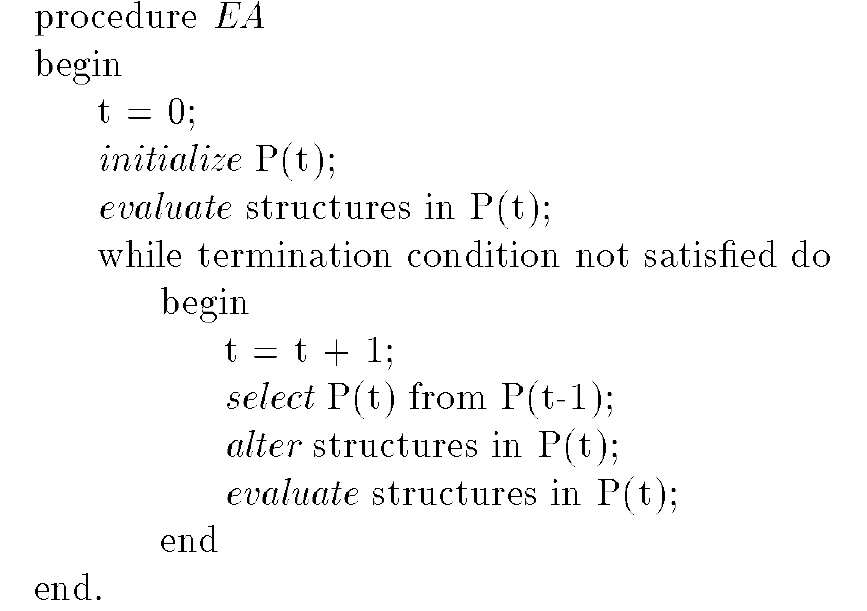
\includegraphics{EA.png}
    \caption{\textit{Pesudo-code Evolutionary Algorithm:} $P(t)$ is the population at time step $t=1,...n$. \texttt{Alter} corresponds to the mutation between populations and \texttt{evalute} corresponds to the measure of fitness of a given population. \cite{Grefenstette99} }
\end{figure}

Breakout is one of the  Atari 2600 games  and is thus an Arcade Learning Environment. This provides a challenging platform for an agent during a reinforcement learning task and is commonly used by the reinforcement learning community as a platform for testing~\cite{Machado17}. Here we see if our NEAT algorithm can learn how to play Breakout and evaluate its performance across generations in python.

\begin{figure}[h!]
    \centering
    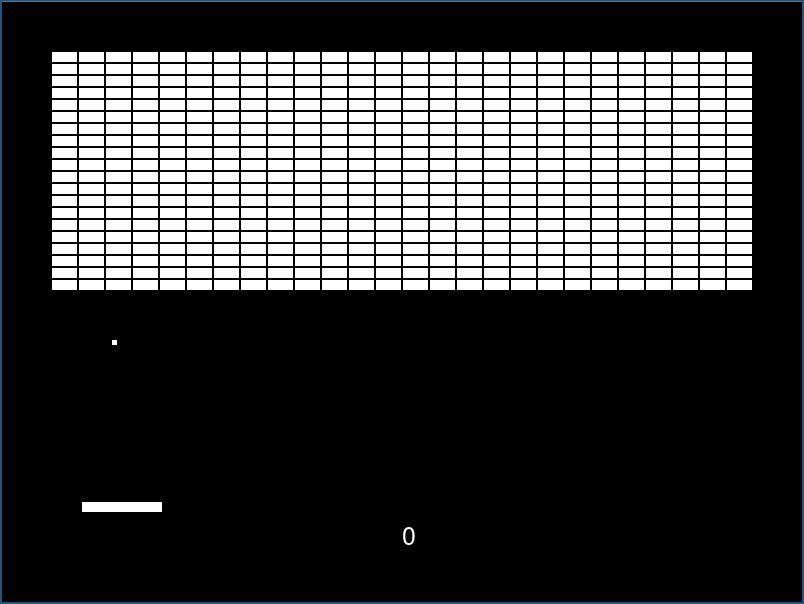
\includegraphics[width=.45\textwidth]{breakout.png}
    \caption{The initial setup of the game Breakout.}
\end{figure}

\section{Results}
We find there are qualitatively three eras of evolution of the network:
\begin{enumerate}
    \item{}\emph{Pre-ball-tracking era}: the network typically does nothing or makes a few small adjustments at the very beginning of the game, scoring a minimal number of points usually $0$ to $30$.
    \item{}\emph{Ball-tracking era}: the network definitively makes an effort to keep the paddle horizontally aligned with the ball. It clears a sizeable portion of the blocks, and only fails in edge cases or by infinitely looping without clearing some remaining blocks. It typically scores $100$ to $400$ points.
    \item{}\emph{Aiming era}: the network tracks the ball as before, but also makes sporadic adjustments to aim at remaining blocks. It clears all or nearly all of the blocks, achieving a score from $515$ to the maximum $520$.
\end{enumerate}
A large percentage of the time, around $90\%$ of attempts, the NEAT algorithm stagnates at a local maximum
fitness somewhere in the first two eras.
Simply repeating the experiment a sufficient number of times eventually yields a trained network that
can achieve the maximum score.
The resultant network is typically very small, having 5 or less non-input nodes and under 15 total connections.
\begin{figure}[h!]
    \centering
    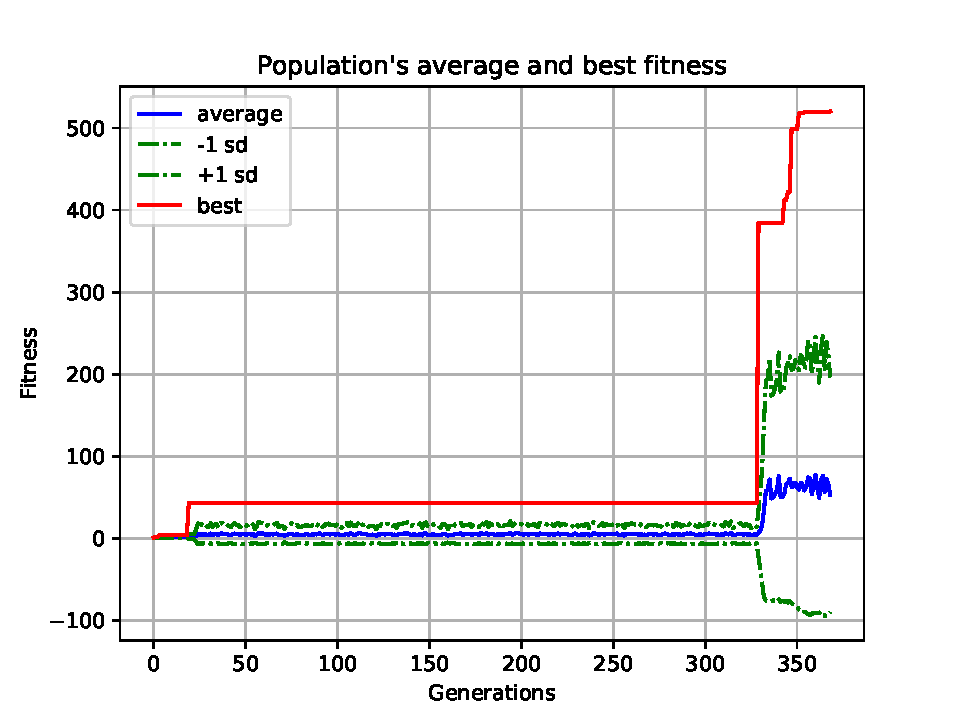
\includegraphics[width=.54 \textwidth]{avg_fitness.pdf}
    \caption{A successful training experiment. In this case, the pre-ball-tracking era lasts
        until around generation 325, where the network abruptly learns how to track the ball.
        The ball-tracking era then lasts until around generation 350, where the network learns to avoid missing stray blocks. The aiming era is eached in the last few generations.
        Generations, each of 200 individuals, took an average time of 2.835 seconds to evaluate running on an
        Intel Core i7-4790K @ 4.00GHz in parallel on 6 cores. The total runtime was around 17.5 minutes.}
\end{figure}

It turned out to be critical to the success of the NEAT algorithm that several previous game states (3 is sufficient) were included as inputs to the neural networks.
Giving only the current state, including the direction of the ball, as input was not sufficient in any
of our experiments to produce a network that could even reliably track the ball.

Another pitfall that was avoided was giving too many inputs to the networks.
If the game state fed to the network
included information about all 520 blocks, then regardless of whether the game history was given,
none of our experiments produced a network that could reliably track the ball.
The vast majority of networks trained in this manner did precisely nothing, making no button presses
at all.
On the other hand, training was able to produce an aiming era individual
when the density of blocks remaining in a few (under 10) predetermined regions were passed as inputs.
Training also succeeded when the game state passed to the networks included no information about the remaining blocks whatsoever, i.e.\ a network that saw only the paddle and ball could still achieve a maximum score.

\section{Methods}
We modified a Pygame~\cite{pygame} implementation of Breakout (cf.~\cite{max00355breakout}) to allow
human mouse input and human keyboard input (for testing purposes), or automated keyboard input.
Then we used NEAT-Python~\cite{neatpython} to run the NEAT algorithm.

To allow the neural network to play Breakout,
each frame a representation of the game state is computed and
passed as the inputs to a neural network.
The neural network has two outputs ``L'' and ``R'', which are binarized
and taken to indicate whether the left or right arrows are being pressed by the neural network.

The representation of the game state includes the following information:
\begin{itemize}
    \item{} the $x$ and $y$ coordinates of the ball, normalized as a percentage of the width of the game
    \item{} the $x$-direction $\pm1$ and $y$-direction $\pm 1$ of the ball,
    \item{} the angle of the ball, normalized as a percentage of $2\pi$
    \item{} the $x$ coordinate of the center of the paddle, normalized as a percentage of the width of the game
    \item{} the history of the previous four up to a fixed number of time steps in the past
    \item{} (potentially) the density of remaining blocks in e.g.\ each of the four block quadrants or similar fixed configuration of predetermined regions of blocks.
\end{itemize}

After carefully choosing the parameters of the algorithm, a neural network
it trained to play Breakout using NEAT with the final score of playing a game being the fitness function.

Since the success of the algorithm is so sensitive to the configuration, we reproduce it here:
\begin{verbatim}
[NEAT]
fitness_criterion     = max
fitness_threshold     = 520
pop_size              = 200
reset_on_extinction   = True

[DefaultGenome]
# node activation options
activation_default      = sigmoid
activation_mutate_rate  = 0
activation_options      = sigmoid

# node aggregation options
aggregation_default     = sum
aggregation_mutate_rate = 0
aggregation_options     = sum

# node bias options
bias_init_mean          = 0.0
bias_init_stdev         = .5
bias_max_value          = 5
bias_min_value          = -5
bias_mutate_power       = .10
bias_mutate_rate        = 0.05
bias_replace_rate       = 0.05

# genome compatibility options
compatibility_disjoint_coefficient = 1.0
compatibility_weight_coefficient   = 0.5

# connection add/remove rates
conn_add_prob           = 0.9
conn_delete_prob        = 0.05

# connection enable options
enabled_default         = True
enabled_mutate_rate     = 0.05

feed_forward            = True
initial_connection      = unconnected

# node add/remove rates
node_add_prob           = 0.1
node_delete_prob        = 0.05

# network parameters
num_hidden              = 0
num_inputs              = 18
num_outputs             = 2

# node response options
response_init_mean      = 1.0
response_init_stdev     = 0.0
response_max_value      = 30.0
response_min_value      = -30.0
response_mutate_power   = 0.0
response_mutate_rate    = 0.0
response_replace_rate   = 0.0

# connection weight options
weight_init_mean        = 0.0
weight_init_stdev       = .5
weight_max_value        = 5
weight_min_value        = -5
weight_mutate_power     = 0.125
weight_mutate_rate      = 0.160
weight_replace_rate     = 0.1

[DefaultSpeciesSet]
compatibility_threshold = 3.0

[DefaultStagnation]
species_fitness_func = max
max_stagnation       = 200
species_elitism      = 1

[DefaultReproduction]
elitism            = 5
survival_threshold = 0.05
\end{verbatim}


\section{Discussions}
What was learned from this experience was largely the difficulty in using genetic algorithms in  neural networks, specifically, evolutionary algorithms for reinforcement learning ~\cite{Grefenstette99} (EARL). For example, the number of generations to reach finish the game may be large. Another issue is in that giving the network such a small set of outputs and forcing it to learn to play a game in such a manner may not be the most pratical approach as this is essentially a random walk on the solution space. There are several future directions for this experment.

We may potentially attempt to redo this experiment with a fixed neural architecture and optimise through stochastic gradient descent on a reward function. specifically, we would implement a deep neural network that optimises a quality function, a deep q network. Such networks have performed empirically better than professionals on games of the Atari 2600 suite, a type of aracade learning environment~\cite{Machado17} that is seen as a baseline for reinforcement learning taks. However, such an approach may offer little insight into the betterment of EARL's. Nevertheless, given that NEAT and DQN's have been demonstrated to perform well on tasks, a comparsion may be of interest to some.

An alternative future direction of exploration would be within the realm of EARLs. The problem is that the problem of optimisation is already hard. Basic questions like what problems are difficult for a genetic algorithm (GA), let alone an EARL, to solve are not well answered~\cite{stejpan09}. This is a problem that we had personally encountered with respect to our optimisitic inital choice of game-- tetris. Tetris proved to be too complex of a solution space for \texttt{NEAT} to reliably learn to navigate. Indeed, after generations, it was not apparent that the network was learning how to play the game.

If one is to flout rigor such as how well an EARL performs with repsect to the heuristic, or the difficulty of the problem, we may also elect to implement a hierarchical representation ~\cite{Liu17}in order to search through the space of possible solutions. Such a hierarchical approach is not only closer to how people generally solve, problems, but has been demonstrated empirically to similar results to networks in the fraction of the time of other EARL's. Nevertheless, the trade off is that instead of learning about EARL's we only learn of a new method that works.




\begingroup
    %\newpage
    \section{References}
    \renewcommand{\section}[2]{}
    \nocite{*}
    \bibliographystyle{abbrv}
    \bibliography{master}
\endgroup
\end{document}
